%Git-rapport
\documentclass[a4paper]{article}

\usepackage[swedish]{babel}
\usepackage[utf8]{inputenc}
\usepackage{graphicx}
\setcounter{secnumdepth}{4}
\usepackage{titlesec}
\usepackage{caption}
\usepackage{float}
%For figures
\graphicspath{ {Figures/} }
\captionsetup{justification=centering}


\begin{document}

\begin{titlepage}
\centering
{\bfseries\huge Projektrapport DAT290}

\vspace{10mm}

{\Large Radiostyrd Bil, Grupp 07}

\vspace{20mm}

{\Large \itshape{Joakim Junttila, Johanna Gudmandsen, Gustav Holst,\\Henrik Klein Moberg, Anders Berggren Sjöblom, \\[1mm] Stanisław Zwierzchowski, Carl Lundgren}}

\vspace{10mm}

%Vet ej vilket datum som ska stå
{DATUM}


\normalsize{
\begin{table}[b]
\centering
\begin{tabular}{|l|l|l|}  \hline
         & \bf Namn & \bf Datum   \\ \hline \hline
Granskad & NAMN     & DATUM        \\ \hline
Godkänd  & NAMN     & DATUM         \\ \hline
\end{tabular} 
\end{table}}
\end{titlepage}

\tableofcontents

\newpage
\noindent {\Large \bf Ordlista}

\vspace{5mm} \noindent
{\bf RF-moduler} - Radiofrekvensmoduler. Är antingen sändare eller mottagare och möjliggör för radiofrekvensiell överföring av bytes~\cite{RFModule}.

\vspace{5mm} \noindent
{\bf PWM-signaler} - PWM eller Pulse Width Modulation är en moduleringsteknik som mest används för att styra mängden elektrisk ström som förs till exempelvis en motor~\cite{PWM}.

\vspace{5mm} \noindent
{\bf Potentiometer} - En elektrisk komponent som med hjälp av ett variabelt motstånd kan begränsa spänning~\cite{Potentiometer}.

\vspace{5mm} \noindent
{\bf ADC} - Analog to digital converter, översätter analoga värden i enheten Volt till digitala värden~\cite{ADC}.

\vspace{5mm} \noindent
{\bf Avståndsmätare} - Mer specifikt, HC-SR04, mäter avstånd från ett objekt med hjälp av ultraljud och dess eko~\cite{DistMeasure}.

\vspace{5mm} \noindent
{\bf ARM} - En processorarkitektur~\cite{chalmersARM}.

\vspace{5mm} \noindent
{\bf UART} - Universal Asynchronous Receiver/Transmitter~\cite{chalmersARM}.


\vspace{5mm} \noindent
{\bf GPIO} - General-purpose input/output~\cite{chalmersARM}.



\newpage
\section{Introduktion}

Radiostyrda bilar började produceras på mitten av 60-talet~\cite{RCHistory}. Under åren har de både tävlats med samt varit en väletablerad leksak. Trots att den genomgått mindre justeringar har den radiostyrda bilens uppbyggnad i det stora hela förblivit densamma.

\subsection{Syfte}

Syftet med detta projekt är att uppdatera den klassiska radiostyrda bilen genom att ersätta befintlig sändare samt mottagare i en radiostyrd bil med nya datorer och även möjliggöra styrning från en Androidtelefon. Avsikten är även att implementera en kontrollapplikation som ska kunna stoppa bilen från att kollidera. Följden av detta blir en produkt mer anpassad till aktuell teknik och det erhålls på så sätt en mer modern teknisk produkt.


%Syftet med detta projekt är att uppdatera den klassiska radiostyrda bilen med hjälp av ny teknik som bluetooth. För att följaktligen erhålla en mer modern teknisk produkt.

\subsection{Mål}
Målen nedan beskriver konkret vad som uppnås med projektet.

\begin{itemize}
\item Den befintliga sändaren samt mottagaren som finns i handkontrollen respektive bilens elektronik byts ut mot ARM-baserade system (se Figur 1). Dessa ska vid färdig produkt kontrolleras via Bluetooth.
\item En kontrollapplikation implementeras. Med hjälp av en avståndsmätare (se Figur 1) är avsikten att bilen ska kunna köra rakt fram i högsta möjliga hastighet och på ett avstånd av maximalt 1 cm från en vägg självständigt bromsa in helt utan att kollidera. Kontrollapplikationen styrs via Bluetooth.
\item Styrning via mobilapplikation realiseras. Bilen kan manövreras genom ett Andriodsystem via Bluetooth.
\end{itemize}

\begin{figure}[H]
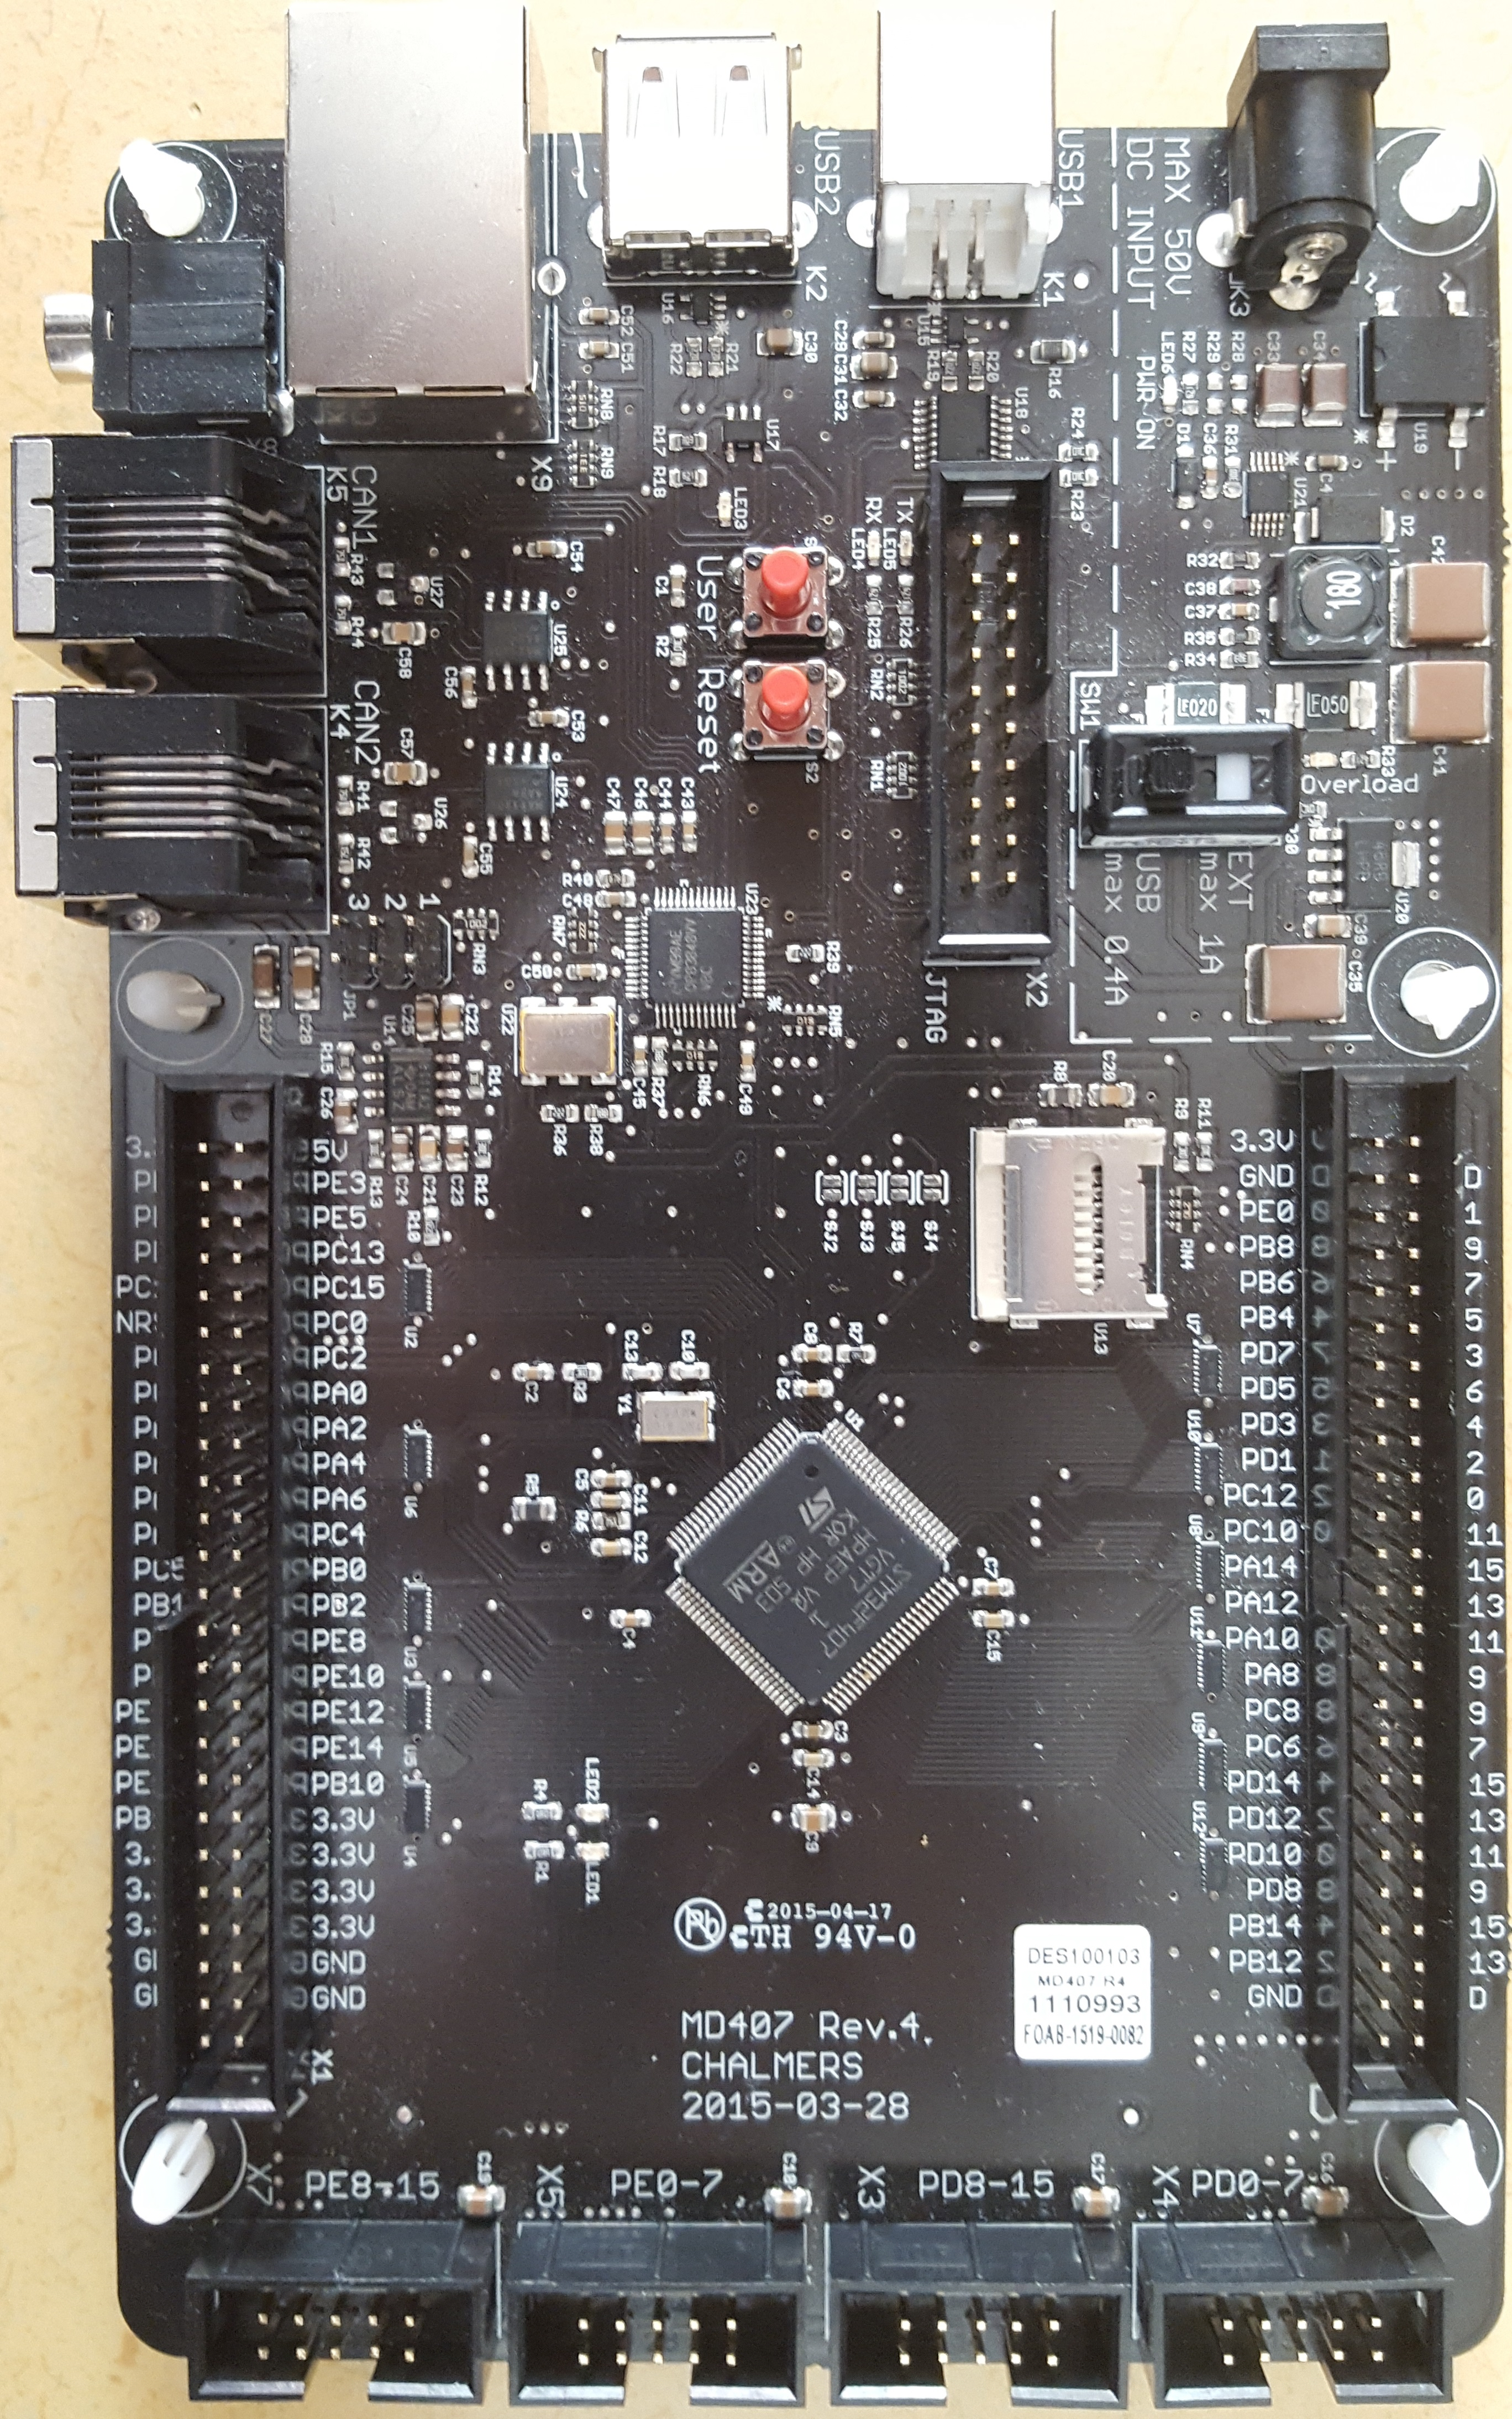
\includegraphics[scale=0.04]{MD407.jpg} \hspace{2mm}
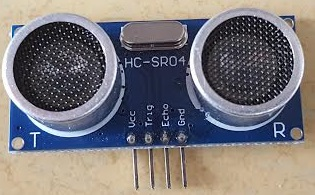
\includegraphics[scale=1]{DistanceMeasurementFront.jpg}
\centering
\caption{\it MD407, en ARM-dator(vänster), Avståndsmätare(höger).}
\end{figure} 

%Målförslag
%Projektet går ut på att ersätta delar av elektroniken i en radiostyrd bil. Sändaren samt mottagaren som finns i handkontrollen ska bytas ut till en ny handkontroll. Nya handkontrollens sändnings singnal kommer ändras till att slutligen bli  Bluetooth. I samband med singnal bytet kommer nya handkontrollen att anpassad till andara ändringar som ska genomföras. Andra ändringar som ker berör bland annat skälva bilen. Bilens elektronik ska bytas ut mot ARM-baserade system. Vidare ska en kontrollapplikation implementeras i bilen med hjälp av ett antal avståndsmätare. Därefter ska bilen programeras så den självständigt ska kunna köra rakt fram i högsta möjliga takt och bromsa in helt på ett avstånd av maximalt 1 cm från en vägg. Sista steget i arbetsprosessen är att med hjälp av Bluetooth signalen utveckla en aplickation som ska kunna styra bilen och fungera som en fullfjädrad handkontroll.

\subsection{Arbetsmetod}
\subsubsection{Uppmätning av styrsignaler}
%VILKET KRETSKORT
Projektet inleds med att mäta upp befintliga styrsignaler. För att kunna återskapa signalerna som skickas från den ursprungliga mottagaren till bilens styrelektronik kopplas ett kretskort, Adapter Maverick, till bilens egna kontrollenhet, MRX-242. Kretskortet har möjlighet att separera mottagarens signaler och kopplat till ett oscilloskop går det att urskilja specifika signaler så de tydligt kan mätas upp. Signalerna är av typen PWM och deras värde bestäms av medelspänningen. 


\subsubsection{Konfiguration av ny mottagare}
En MD407-enhet ersätter mottagaren i bilen. Kanalerna CH3 och CH4 på det integrerade timer-kretskortet, TIM2, konfigureras för att hanteras av portarna PA2 respektive PA3 i C-koden. Koden, utvecklad i Codelite, initierar CH3 till att reglera motorstyrningen och CH4 till att kontrollera rattutslagen. Följden av detta blir att portarna PA2 och PA3 i den ersättande mottagaren kopplas direkt till bilens styrelektronik, en kabel till motorn och en till styrservot. 

\vspace{5mm} \noindent
Information tas emot genom radiofrekvensmoduler. När RF-mottagaren erhåller ett meddelande triggas en funktion i koden. Denna ska undersöka vilket kommando som ska utföras samt till vilken grad detta skall göras enligt bitarnas anvisningar i Figur 2. Värdet 1 eller 2 på kommandobitarna leder till att bilens motor eller styrservo påverkas i angiven ordning. Tar mottagaren exempelvis emot kommandot att bilen ska ändra motorhastigheten skickas denna information till motorns styrelektronik. Den nya hastigheten beror på storleken av värdet. Värdet på meddelandet från sändaren skickas som en PWM-signal till den begärda styrelektroniken i bilen som fångar upp dessa under en period(se exempel i Figur 3), uppfattar värdet och agerar. Detta arbete har förenklats med hjälp av kodbibliotek från STMicroelectronics som innehåller funktioner för att initiera PWM-genererande. Observera att bilen endast svarar korrekt på värden där PWM-signalen är hög under ungefär 8\%-12.4\% av perioden, en högre eller lägre andel än detta kan få elektroniken att överbelastas. Värden i meddelanden mellan RF-modulerna kan antas från 0-63, utifrån 6 bitar, och TIM2 konfigureras därför till att addera en offset av 110 innan PWM-signalen skickas till styrelektroniken för att möjliggöra för korrekt avläsning.



\begin{figure}[H]
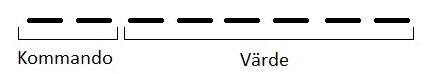
\includegraphics[scale=1]{aByteComVal.jpg}
\centering
\caption{\it Specifikationer av byten som seriellt skickas från sändare till mottagare.}
\end{figure} 


\begin{figure}[H]
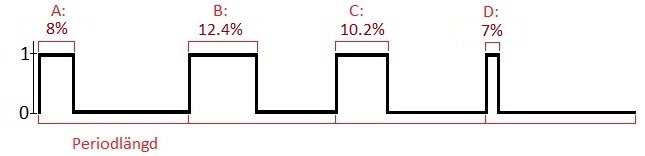
\includegraphics[scale=1]{PWMsignals.jpg}
\centering
\caption{\it Exempel på möjliga PWM-signaler. Om byten indikerar att motorn ska påverkas kommer den i fall A och B köra i högsta fart baklänges respektive framlänges. I fall C hamnar bilen i neutralt läge och står då stilla. Signalen i fall D tolkas ej av bilens styrelektronik då det ligger utanför dess avläsningsintervall.}
\end{figure} 



\subsubsection{Konfiguration av ny sändare}
En datorenhet, MD407, ersätter sändaren. Potentiometern kopplas enligt anvisningar från Figur 4 och även sedan till MD407 via en flatkabel för strömförsörjning enligt tidigare nämnd figur. Kablarna som kopplas till datorenheten sätts på PC1-porten och PC2-porten på MD407 i angiven ordning från figuren. De reglerar hastigheten respektive rattutslaget. Initiering av detta skrivs i C med utvecklingsmiljön Codelite.


\begin{figure}[H]
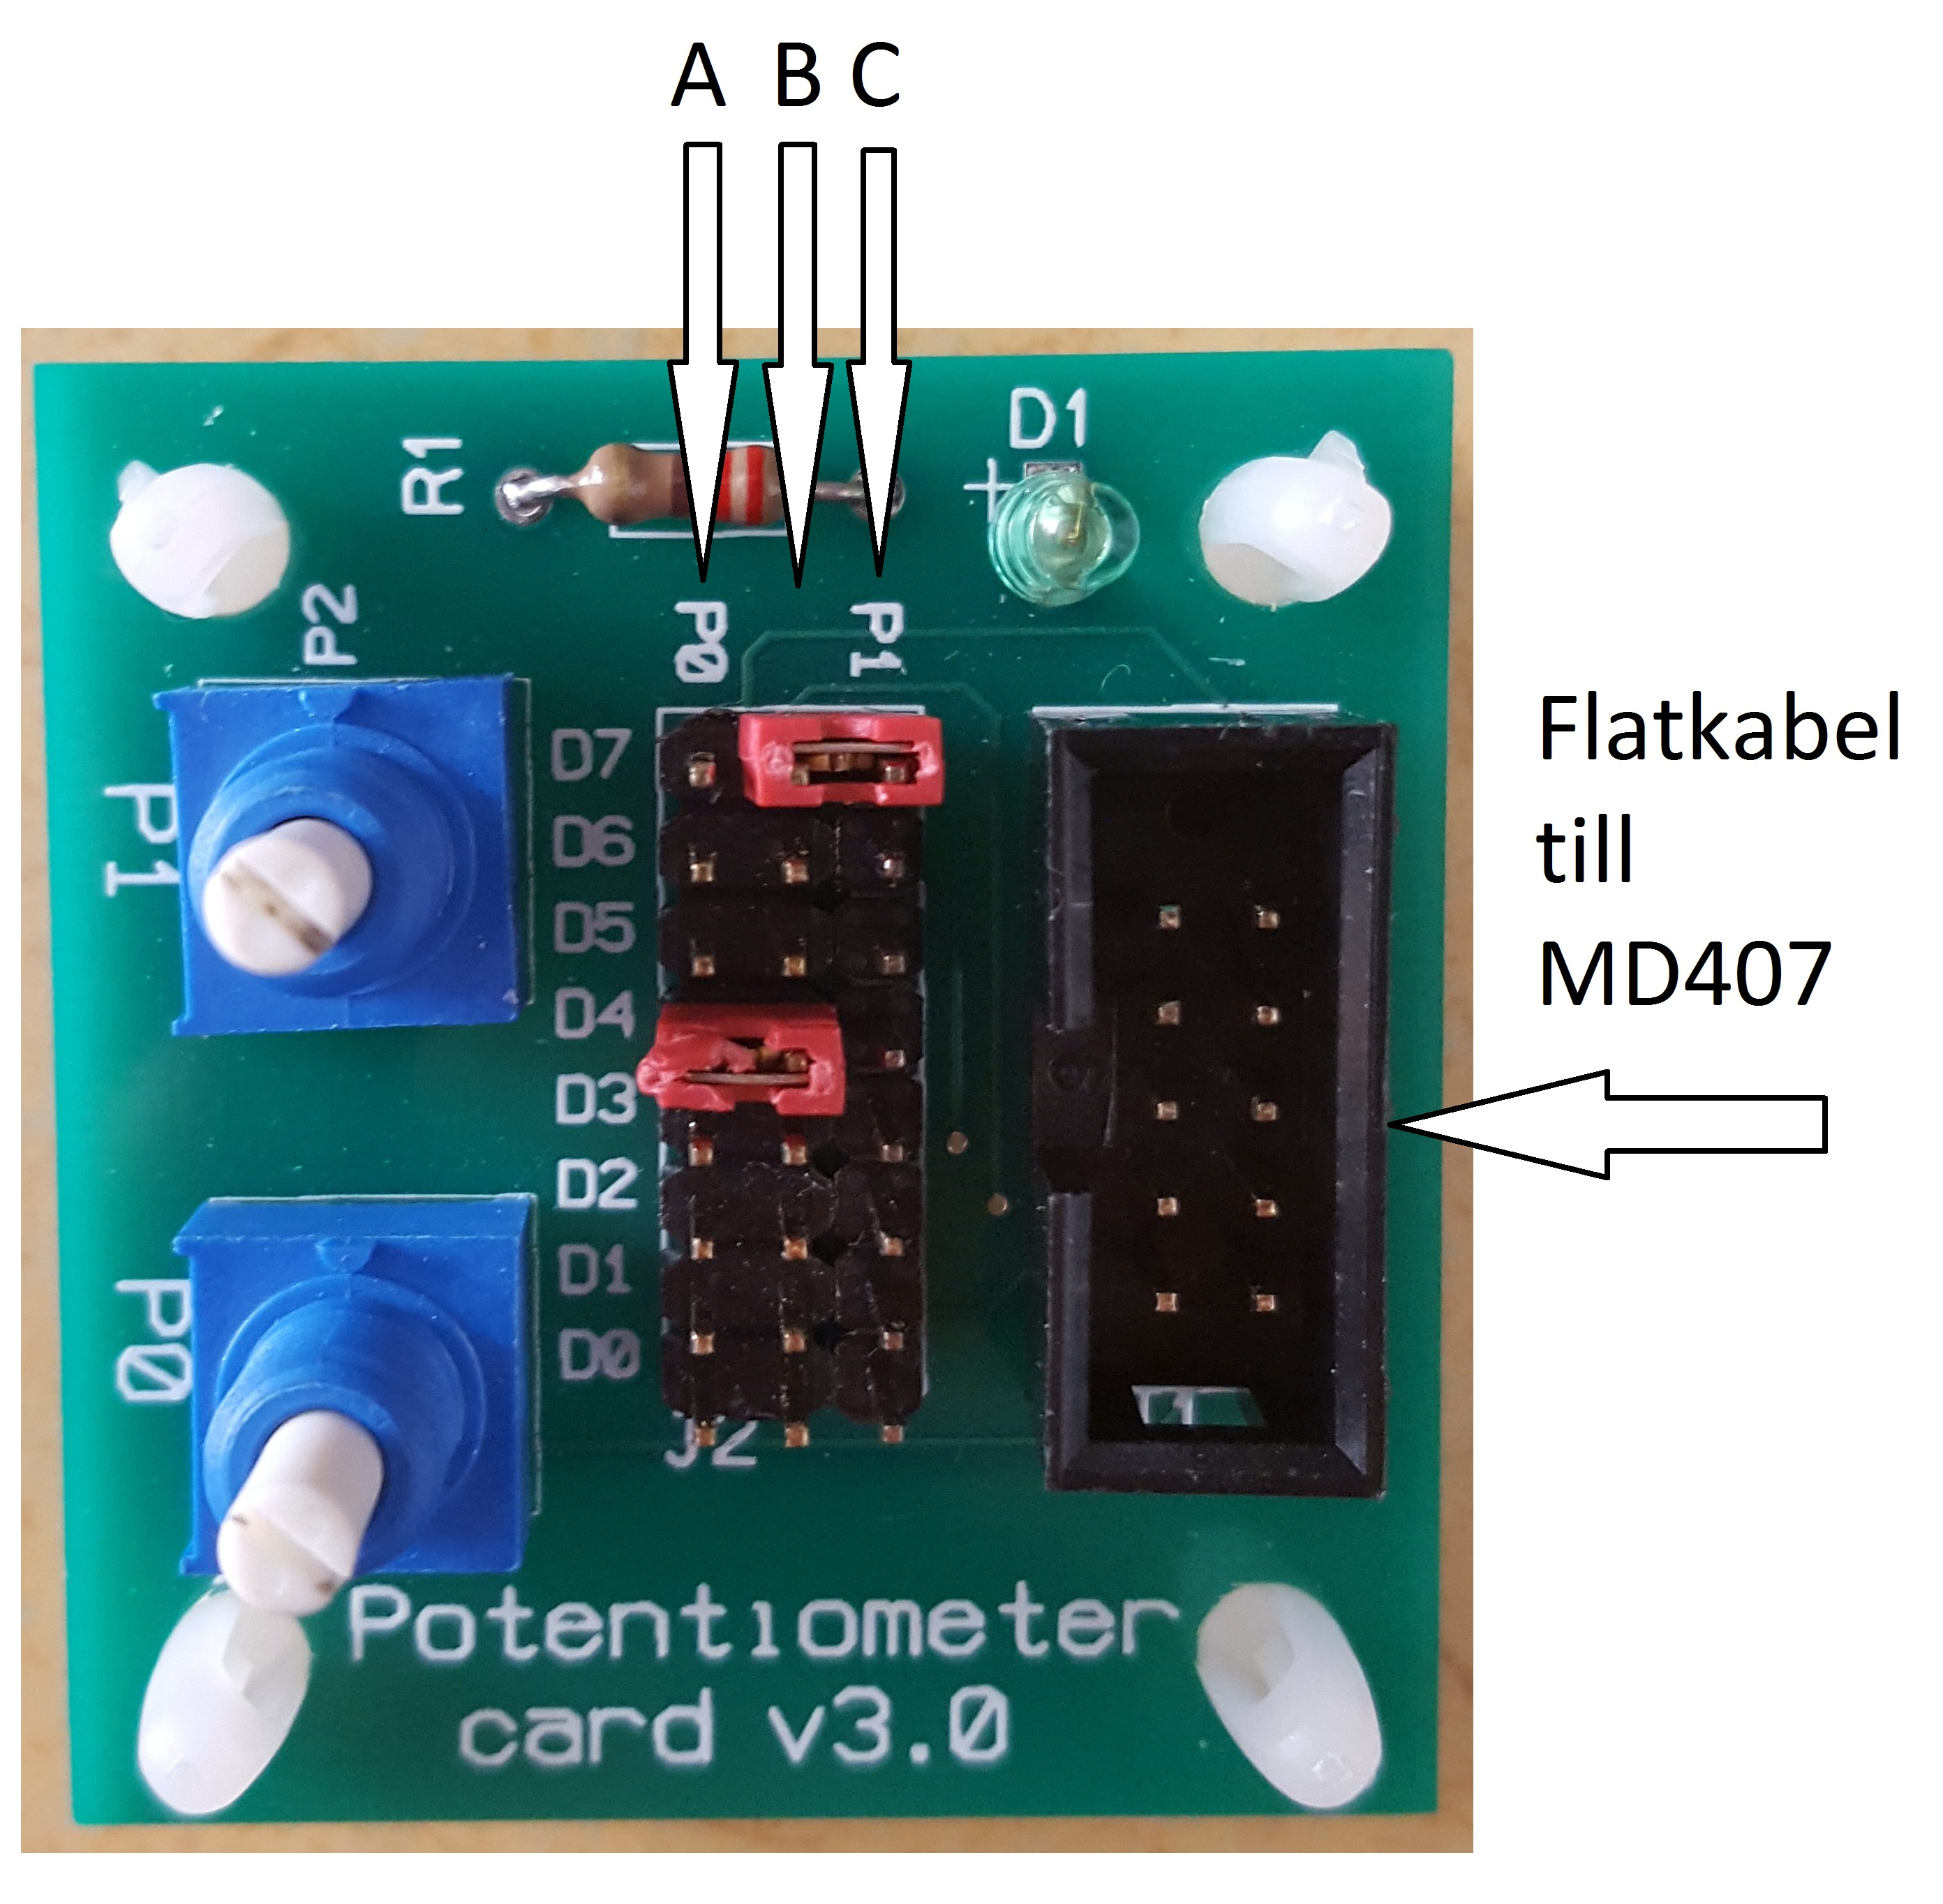
\includegraphics[scale=0.05]{PotentiometerMedRitning.jpg}
\centering
\caption{\it En potentiometer. A, B och C representerar kolumner. B leder ström och kopplas till A respektive C med kort kabel såsom bilden visar. För att få värden till datorenheten kopplas även en kabel från A, rad 1, och C, rad 4, till MD407}
\end{figure} 

\subsubsection{Sändare och mottagare kopplas samman}
Båda datorenheterna kopplas samman. Med hjälp av programmet ETERM kan USART genom USB koppla två bärbara datorer till sändare och mottagare för att ladda upp kompilerad C-kod till MD407-enheterna som då kan utföra operationer utifrån koden. PA0-porten på sändaren initieras till kretskortet UART4 som i sin tur kopplas till en RF-sändare på DATA-pinnen. UART4 kan då skicka data via PA0 till RF-modulen. En identisk procedur görs på mottagaren men på PB11-porten med kretskortet USART3 och en RF-mottagare. Resterande inkopplingar av RF-modulerna görs enligt Figur 5. Koden påbörjar därefter att seriellt skicka bytes med information från sändarens potentiometer till mottagarens enhet för avläsning. Viktigt är att koden initierar bytes att skickas från sändaren ungefär 100 gånger i sekunden för att minska störningar och få värdeövergångarna att bli så jämna som möjligt. Stöd från hjälpfunktioner i bibliotek möjliggör för att kunna skriva till PA0-porten och läsa från PB11-porten. Koden är utvecklad i Codelite.

\begin{figure}[H]
\includegraphics[scale=0.06]{RF-transmitter.jpg}
\includegraphics[scale=0.05]{RF-receiver.jpg}
\centering
\caption{\it 4-pin RF-sändaren (vänster) och 3-pin RF-mottagare (höger). GND kopplas till datorenheternas GPIO-portar för jord och VCC till deras 5V-portar.}
\end{figure} 


\subsubsection{Komplettering med applikation som sändare}
Mobilapplikationen ska vara funktionell på en Androidtelefon och kopplas till den radiostyrda bilen via Bluetooth. Två applikationer konstrueras separat; en GUI, grafiskt användargränssnitt, med olika reglage för att styra hastighet och riktning, samt en applikation som kontrollerar Bluetooth. Dessa skrivs i Java genom Eclipse och importeras till Android Studio, en utvecklingsmiljö för Andriodapplikationer. Sedan sammanställs dessa till en applikation för att genom den kunna koppla sin Bluetooth-modul med MD407-mottagaren och på så vis skicka värden till bilen.

\newpage
\section{Teknisk beskrivning}

\subsection{Teknisk bakgrund}
För att kunna kontrollera en radiobil används en RF-sändare och en RF-mottagare ~\cite{RCTechnique}. Radiosignaler skickas från RF-sändaren och avkodas av RF-mottagaren i radiobilen, de kommunicerar över 2.4GHz-bandet. Dessa omvandlas då till elektroniska signaler som antingen kontrollerar bilens hastighet eller riktning. Parallellt med detta styrs även bilens hastighet, framåt eller bakåt, av motorns kraftutslag, medan riktningen beror på hjulens gradförskjutning. Bilens styrenhet omvandlar radiosignaler som sedan kontrollerar bilens rörelse.

\subsubsection{Styrsignaler}
Bilens styrsignaler kontrolleras av en kontrollenhet, MRX-242~\cite{projektDir}. Enheten fungerar simultant som radiomottagare och styrsignalsgenerator. Den genererar signaler till båda motorerna i bilen via tre kablar. I mening att replikera dessa finns även tillgång till ett ytterligare kopplingsblock.


\subsection{Systemöversikt}
Systemet har två huvuddelar, en MD407-enhet samt en Androidapplikation som båda kan agera handkontroll, och en MD407-enhet som genererar signaler till motorerna.

\subsubsection{Styrning från MD407 till MD407}
\begin{figure}[H]
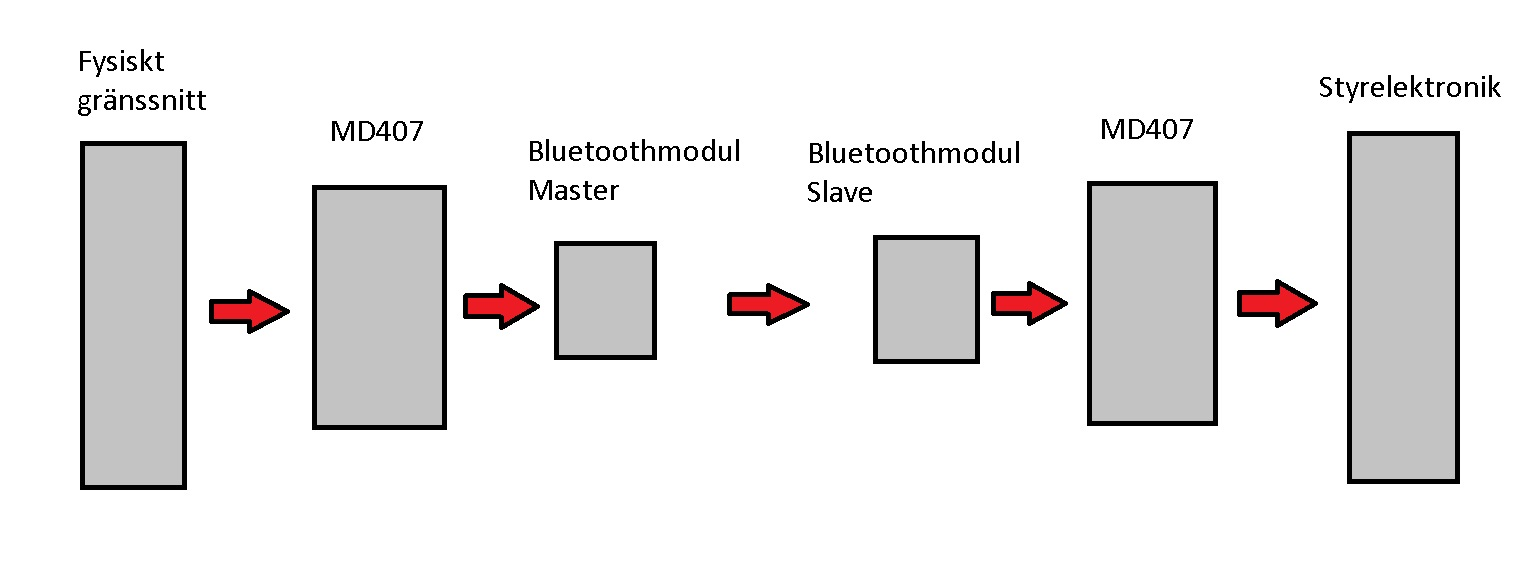
\includegraphics[width=\textwidth]{systemoversikt.jpg}
\centering
\caption{\it En översikt över systemet i blockformat med MD407 till MD407. Pilarna indikerar flödet av information, analogt eller digitalt.}
\end{figure} 


%KOLLA SÅ ATT DET ÄR BLUETOOTH OCH INTE RF
Enligt Figur 6 erhålls en överblick över hur systemet fungerar. Den sändande datorenheten MD407 får information från en potentiometer och skickar dessa värden via Bluetooth till den mottagande MD407-enheten som tar emot värdena och överlämnar dessa till bilens styrelektronik som agerar efter dem.

\subsubsection{Styrning från Androidapplikation till MD407}
\begin{figure}[H]
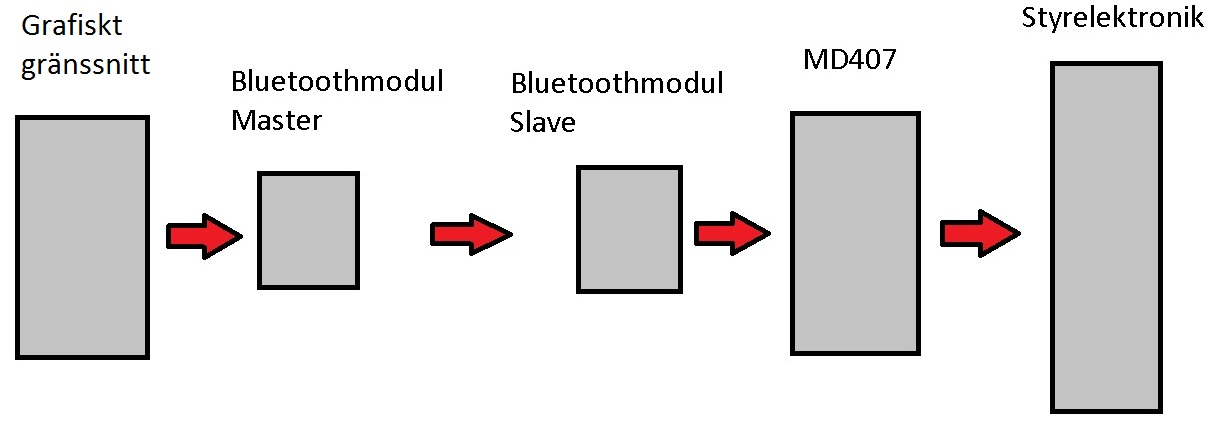
\includegraphics[width=\textwidth]{systemoversiktAndroid.jpg}
\centering
\caption{\it En översikt över systemet i blockformat med Androidapplikation till MD407. Pilarna indikerar flödet av information, analogt eller digitalt.}
\end{figure} 

Figur 7 visar en sammanfattning över systemet med en applikation som sändare. Observera att skillnaden mellan den tidigare styrningen är att Androidapplikationen skickar bytes genom sin integrerade Bluetooth-modul till mottagarens inkopplade. På samma sätt som tidigare analyseras sedan värdena och skickas till bilen.


\subsection{Delsystem}
\subsubsection{Specifikation av nya styrsignaler}
Bilen uppfattar PWM-signaler 72 gånger i sekunden. De ursprungliga signalerna skickas på en frekvens av 72Hz, i mening att replikera dessa ges TIM2s räknare en frekvens av 100kHz. Ett antal klockcykler divideras med denna frekvens och kvoten ska då hamna nära 1/72. Antalet klockcykler är således bestämda till 1388. Resultatet av detta är att de nya PWM-signalerna skickas 72 gånger i sekunden till bilen som styrelektroniken läser av.

\vspace{5mm} \noindent
PWM-signalerna kan endast avläsas korrekt av styrelektroniken på specifika värden. I varje period under en PWM-signal kan spänningen antingen vara 0, låg, eller 1, hög. Det som bilens styrelektronik svarar på är hur stor del av perioden signalen är hög (se Figur 3),  alternativt hur stor del av signalen som sänder 3.4V. Medelspänningen vid styrning och hastighet när styrningen är maximalt åt vänster respektive höger och hastigheten är maximalt bakåt respektive framåt går från 269mV till 423mV. Bilen når således högsta möjliga vänsterlutning samt fart bakåt vid 269mV, neutralt läge vid 348mV och maximal högerlutning samt fart framåt vid 423mV. Genom att dividera dessa värden enskilt med den maximala spänningen, som kan skickas från pinnarna på MD407, och sedan multiplicera med perioden, erhålls det värde bilens styrelektronik läser av. Detta resulterar i att bilen lyssnar på värden mellan 110-173 klockcykler under en period av 1388 klockcykler, det vill säga en andel av ungefär 8\%-12.4\% av hög signal. Detta styrs i bilen med hjälp av datorenhetens tidsmekanismer och dess standardbibliotek.

\subsubsection{Sändare: Androidapplikation}
Androidapplikationen agerar som en handkontroll. Denna skickar bytes seriellt till bilens dator via en Bluetooth-länk. Detta följer samma protokoll som tidigare nämnts där de 2 mest signifikanta bitarna i varje byte bestämmer vilken sorts signal som ska ändras och de resterande bitarna bestämmer med vilket värde detta ska ske. Mobilapplikationen har på skärmen virtuella reglage (se Figur 8) som ska emulera ordinarie handkontrollens analoga funktion så att exempelvis hastighetsövergången är så jämn som möjligt.

\begin{figure}[H]
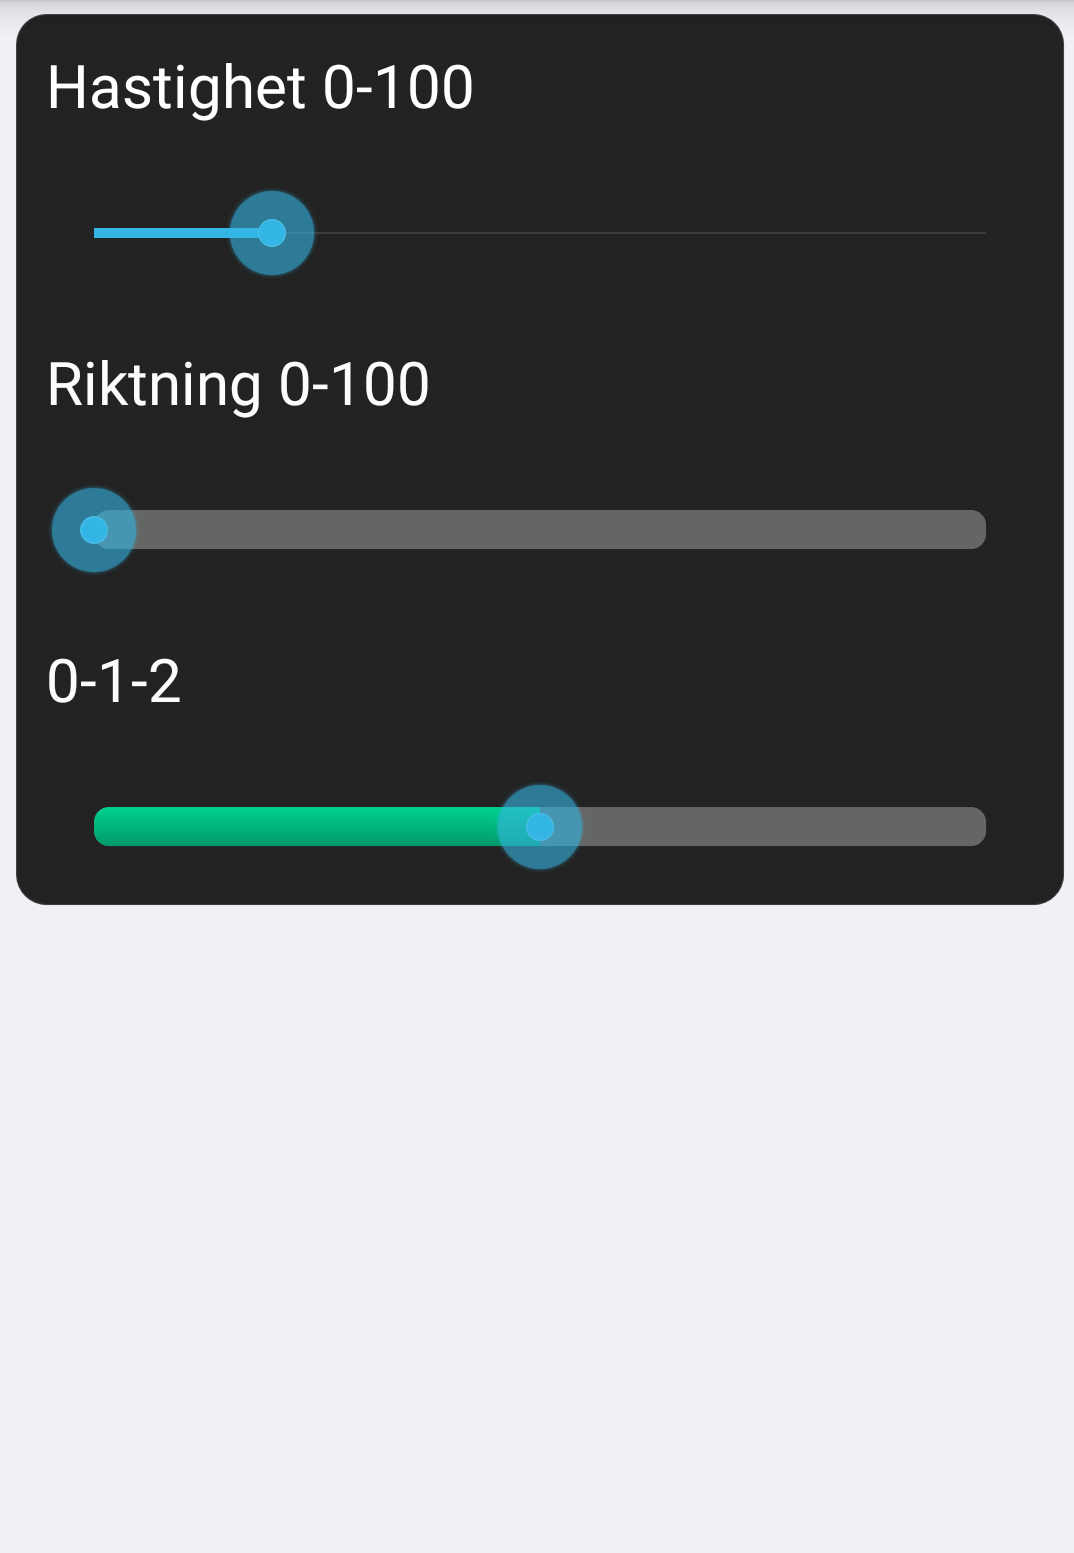
\includegraphics[scale=0.2]{applikation1.png}
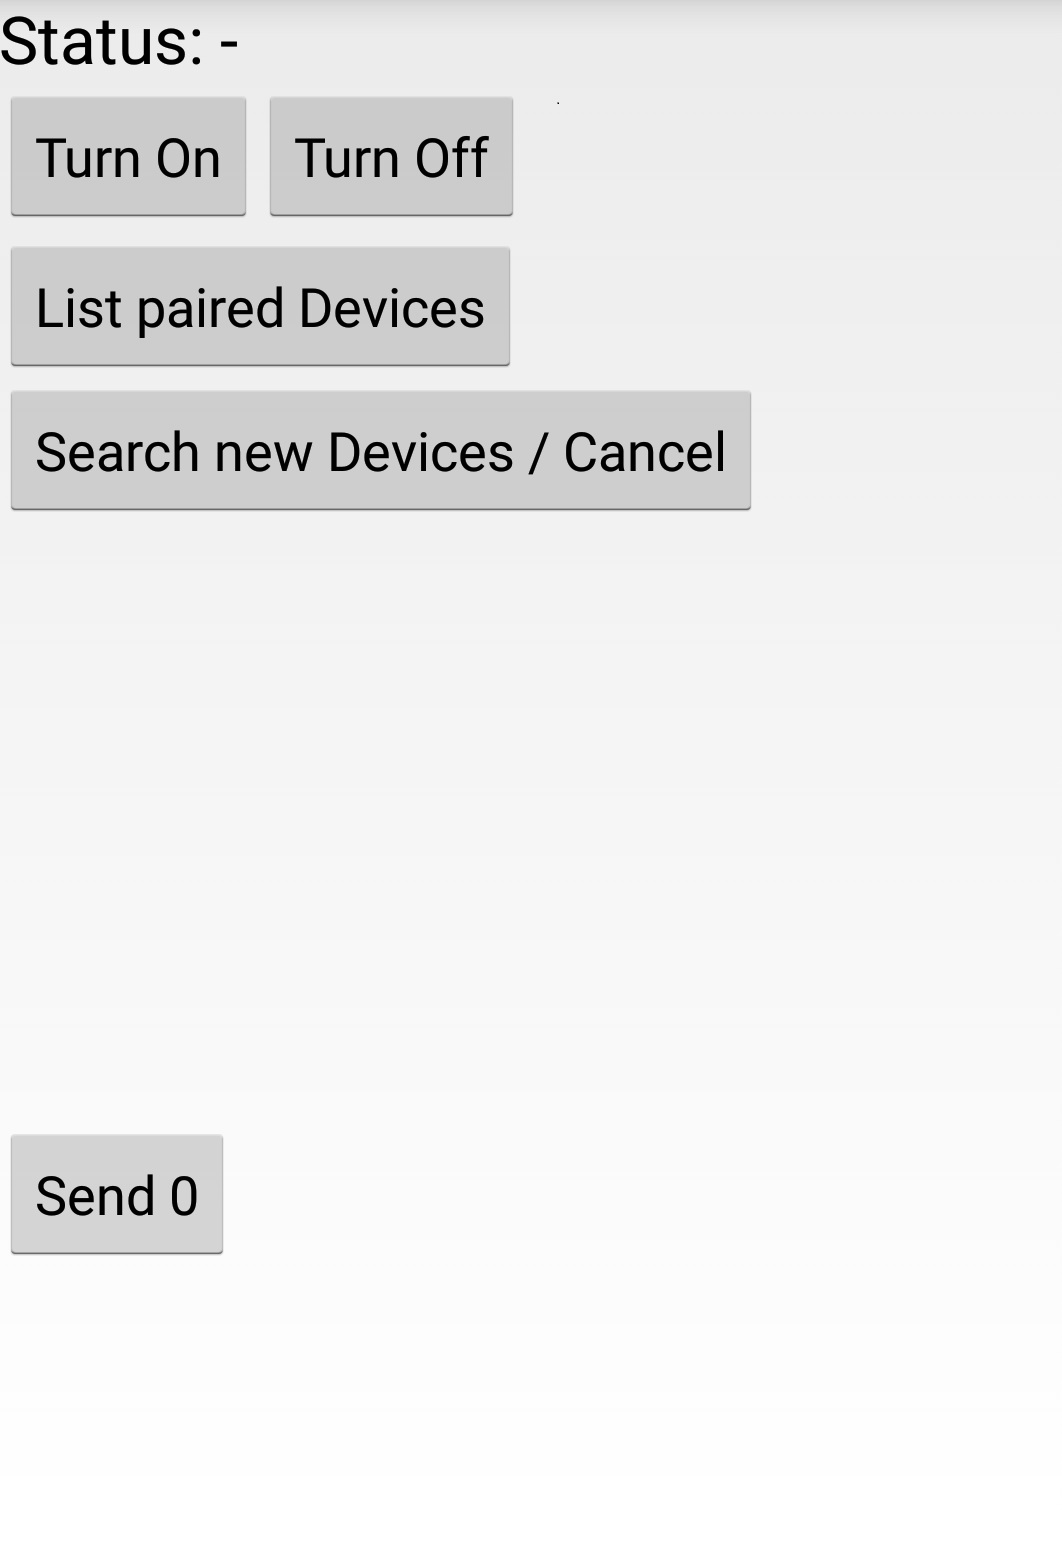
\includegraphics[scale=0.2]{applikation2.png}
\centering
\caption{\it Applikationens virtuella reglage (höger) samt applikationens Bluetooth-gränssnitt (vänster).}
\end{figure} 

\subsubsection{Sändare: MD407-enhet via RF}
Datorenheten MD407 skickar värden från potentiometern till mottagaren. MD407 försörjer dess inkopplade potentiometer med ström och läser konstant av PC1-porten och PC2-porten som i metoden nämndes vara kopplade till potentiometerns utmatningar. På datorenheten finns en integrerad ADC, vilken tar emot värdena från potentiometerns utmatningar och översätter dessa till digitala värden. Resultatet skickas seriellt i bytes från sändarens RF-modul och avläses i mottagarens RF-modul varpå mottagardatorn svarar direkt till styrelektroniken såsom byten specificerar.


%De tre kolumnerna av pinnar som finns i mitten på potentiometern(se Figur 2) använts till olika ändamål. Den mittersta kolumnen möjliggör för ström, därav får de vridbara kontakterna på potentiometern ström genom de korta sladdarna mellan strömkolumen till respektive vridkontakt. Sladden från den sista kolumnen på samma rad kopplat till MD407 ger värden konstant till datorenheten. På denna enhet finns en integrerad ADC. Denna tar emot värdena från portarna PC1 samt PC2 och översätter det till digitala värden. Genom RF-moduler kan de nya datorenheterna kommunicera. Resultatet skickas från sändarens RF-modul en byte åt gången 100 gånger i sekunden till mottagarens RF-modul. Specifikationerna som följs är att de första 2 bitarna indikerar kommandot och de resterande 6 bitarna med vilket värde kommandot ska utföras. 

\subsubsection{Mottagare: MD407-enhet}
%Byt it till: ((((generisk Bluetooth-modul som är kopplad till USART1-porten))) när bluetooth kommer
Signalerna som sändaren skickar hanteras av mottagarens datorenhet. När programmet på denna dator påbörjas måste datorn initialt skicka PWM-signaler som motsvarar neutralt läge för drivmotorn i en kort stund innan övriga signaler kan sändas. Efter detta kan mottagaren ta emot bytes från sändaren genom sin RF-mottagare, samt skicka PWM-signaler till bilens styrelektronik. Byten analyseras då i mening att skicka en PWM-signal till korrekt elektronik i bilen. Som tidigare nämnts har de 6 minst signifikanta bitarna ett värde mellan 0-63 när mottagaren får dem. Till detta adderas en offset av 110 vilket gör att värdet istället kommer befinna sig i intervallet 110-173. Detta värde motsvarar andelen av perioden 1388 där PWM-signalen till bilens styrelektronik kommer vara hög, som i sin tur motsvarar en viss medelspänning bilens styrelektronik direkt agerar på. Bilen svarar därefter med korrekt funktionalitet. Syftar kommandot exempelvis på motorn (se Figur 9) kommer bilen åka i högsta möjliga hastighet bakåt vid värdet 110. Farten minskar sen vid högre värden och bilen når neutralt läge vid 142. Värden över detta upp till 173 får bilen att öka farten. Uppfattar bilen värden utanför detta intervall kan en överbelastning av bilens elektronik ske. 

%Utöver detta kan en kontrollapplikation påbörjas(FORTSÄTT VID MER INFO). 

\begin{figure}[H]
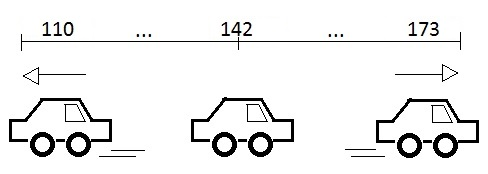
\includegraphics[scale=1]{110-173Car.jpg}
\centering
%SE ÖVER CAPTION, DENNA TEXT ÄR NÄMND I TEXTEN OVAN, ONDIG DÅ KANSKE
\caption{\it Bilen uppnår maximal fart bakåt vid ett värde av 110 och minskar hastigheten tills den når stillastående läge, värde 142. Sedan börjar den accelerera tills den når sin maximala hastighet framåt vid värde 173.}
\end{figure} 



%Datorn i bilen tar då emot ett kommandokod från Bluetooth-länken och analyserar detta i mening att specificera vilket kommando de två bitarna syftar på ska utföras. PWM-signalerna ändras sedan efter värdet på kommandot, de sex minst signifikanta bitarna, eller påbörjar kontrollapplikationen för demonstration. Motorerna tar emot PWM-signalerna och ger utslag beroende på deras medelspänning.






\newpage
\section{Resultat}






\newpage
\section{Slutsats och diskussion}



\newpage
%To references
\bibliographystyle{IEEEtran}
\bibliography{referenserRapport}


\end{document}

